\subsection{VANET - Vehicular Ad Hoc Networks}

VANET - is a network that combines V2V (Vehicle-to-vehicle) and V2I (Vehicle-to-infrastructure) communication.\par
% 
\begin{figure}[h]
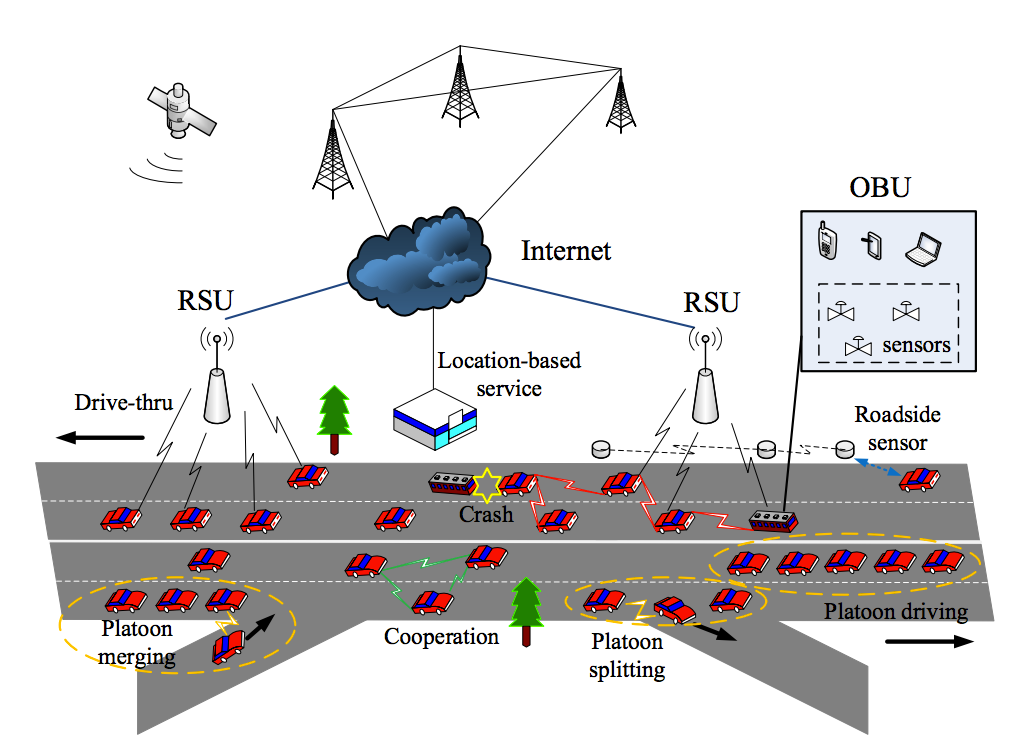
\includegraphics[width=\textwidth]{VANET}
\caption{VANET formation. Figure taken from \cite{Jia2016ASystems}.}
\centering
\label{fig:VANETformation}
\end{figure}
% 
It is large and complex network where vehicles exchange data between each other and any other infrastructure on the road. Traffic participant might receive data, that will prevent accident from happening, relayed from multiple interconnected nodes. Generally VANETs introduce:

\begin{itemize}
    \item Safer and more efficient roads
    \item Logistics, transport and service business improvement
    \item Controlled congestion, more comfortable travelling.
\end{itemize}

One main disadvantage that slows down VANET development that it is dependant on expensive road infrastructure\footnotemark.\par
% 
\footnotetext{\url{http://wifinotes.com/mobile-communication-technologies/what-is-vanet.html}, accessed on 19/04/2017}
% 
VANET is based on latest mobile communication technologies. Following chapters will discuss present and upcoming technologies that would benefit this project.

\subsubsection{V2V}

/Michal's section

V2V communication is a vehicle-to-vehicle communication, where vehicles can communicate with each other and share vital information. In last decades, a lot of research has been done in field of V2V, in which different companies, institutions or organisations participated (either as part of project or on their own). This led to creation and adaptation of standards so that developed technologies by different companies can communicate without difficulties. For the short-range communication IEEE 802.11p standard is adopted which is a wireless protocol (similar to Wi-Fi), operating on 5.85-5.925 GHz (depending on country).

\subsubsection{V2I}
% 
Vehicle-to-Infrastructure technologies are still under development, but it has great potential. Its main idea is communication with vehicle by any road side unit (e.g. traffic lights, road sensors) to prevent accidents and improve road efficiency.\par
% 
% Vehicle-to-Infrastructure Technologies Expected to offer Benefits
\begin{figure}[h]
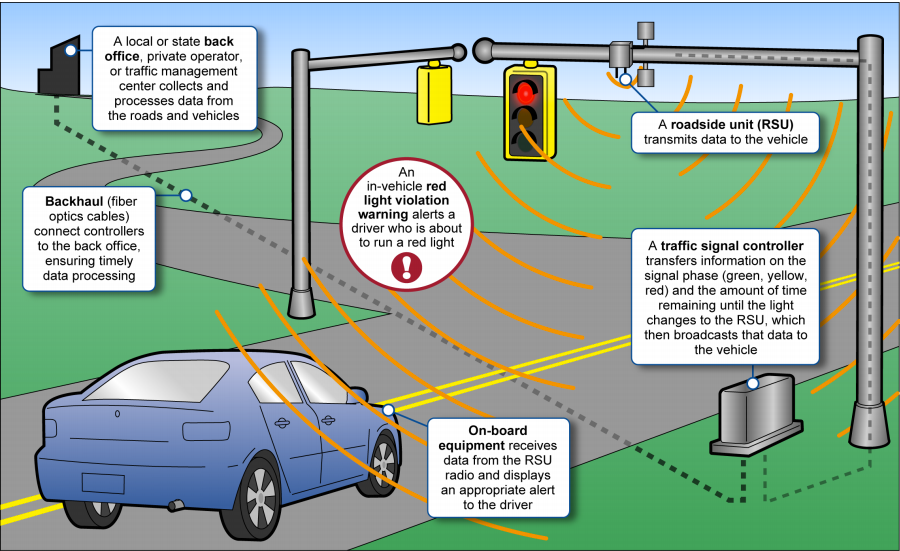
\includegraphics[width=\textwidth]{V2I}
\caption{V21 implementation. Taken from \cite{U.S.GovernmentAccountabilityOffice2015IntelligentExist}.}
\label{fig:V2Iimplementation}
\centering
\end{figure}
% 
There no standards yet of what V2I system architecture should consist of. Architecture framework defined by USDOTs' ITS Joint Program Office \cite{Dr.Gaspar2014HighlySystems} states, that minimal parts for V2I system are:
\begin{itemize}
    \item Vehicle On-Board Unit
    \item Roadside Unit
    \item Safe Communication Channel.
\end{itemize}
% 
Communication is based on 802.11 standard by IEEE, which will be discussed in detail in following chapters. A frequency spectrum in 5.9 GHz range was allocated for exact means in U.S. and Europe \cite{2011TheTechnology}. Although, there are some concerns sharing allocated spectrum, since Middle Class Tax Relief and Job Creation Act of 2012 allowed use of 5.9GHz spectrum for any unlicensed devices and that could cause harmful interference for sending and receiving data in V2I communication \cite{U.S.GovernmentAccountabilityOffice2015IntelligentExist}.\par
% 
Despite any concerns, Vehicle-to-Infrastructure is quickly developing and gaining a lot of attention from scientists and businessman worldwide.\par
%
//To be restructured.
% 
\begin{figure}[h]
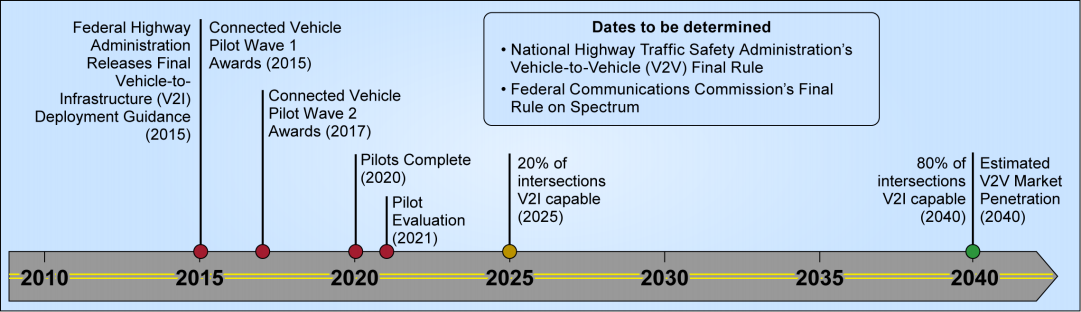
\includegraphics[width=\textwidth]{V2Xtimeline}
\caption{V21 development path. Taken from \cite{U.S.GovernmentAccountabilityOffice2015IntelligentExist}.}
\label{fig:V2Idevelopment}
\centering
\end{figure}


\subsubsection{802.11}
% 
When wireless networks first came around, it was expected that the radio medium will only be another physical layer, such as cables. However, it did not take long to see that due to significant differences of radio communication, more detailed, radio-suited standard needs to be developed. In 1991 work has begun in preparation of standard that is today known as \emph{802.11} \cite{Hiertz2010TheUniverse}. The scope of this standard is \textquote[\cite{2016IEEEAccess.}]{\emph{to define one medium access control (MAC) and several physical layer specifications for wireless connectivity for fixed, portable, and moving stations within a local area.}}\par
One of the most well-known implementations of 802.11 is Wi-Fi. Naturally, it is not the only one and over the years, several amendments have been accepted to initial standard, to accommodate various needs. As Bilgin\&Gungor \cite{Bilgin2013PerformanceAreas} suggest, amendment 802.11b may be used in vehicular environment. Furthermore (and more importantly), amendment 802.11p has been published in 2010. This amendment is designed for the use in transportation, where communication window between two entities may only exist for very limited amount of time and thus some authentication procedures need to be omitted. We will discuss both amendments in following sections.
% 
% 
% 
\subsubsection{802.11b}
% 
The 802.11b uses the 2.4GHz unlicensed spectrum and provided increased maximum data rate of 11 Mb/s. It  modulates the data with spread spectrum modulation technique \emph{Direct-sequence spread spectrum} (DSSS). The spread spectrum modulation modifies the signal in a way, that broader spectrum is used than necessarily needed before modulation. Since the signal is spread over more frequencies, it is less vulnerable to interference \cite{MaximIntegratedProductsInc.2013AnMaxim}.
Similarly to the original standard, 802.11b uses the \emph{Distributed coordination function} (DCF) as the Medium access control (MAC) \cite{Hiertz2010TheUniverse}. DCF is a protocol that utilises \emph{Carrier-sense multiple access with collision avoidance} (CSMA/CA) together with binary exponential back-off algorithm. The CSMA/CA listens for broadcast on a channel and if there is none (of the channel is free) only then it starts broadcasting. The operation of CSMA/CA can be seen in detail in figure \ref{fig:csma-ca}.
% 
\begin{figure}
    \centering
    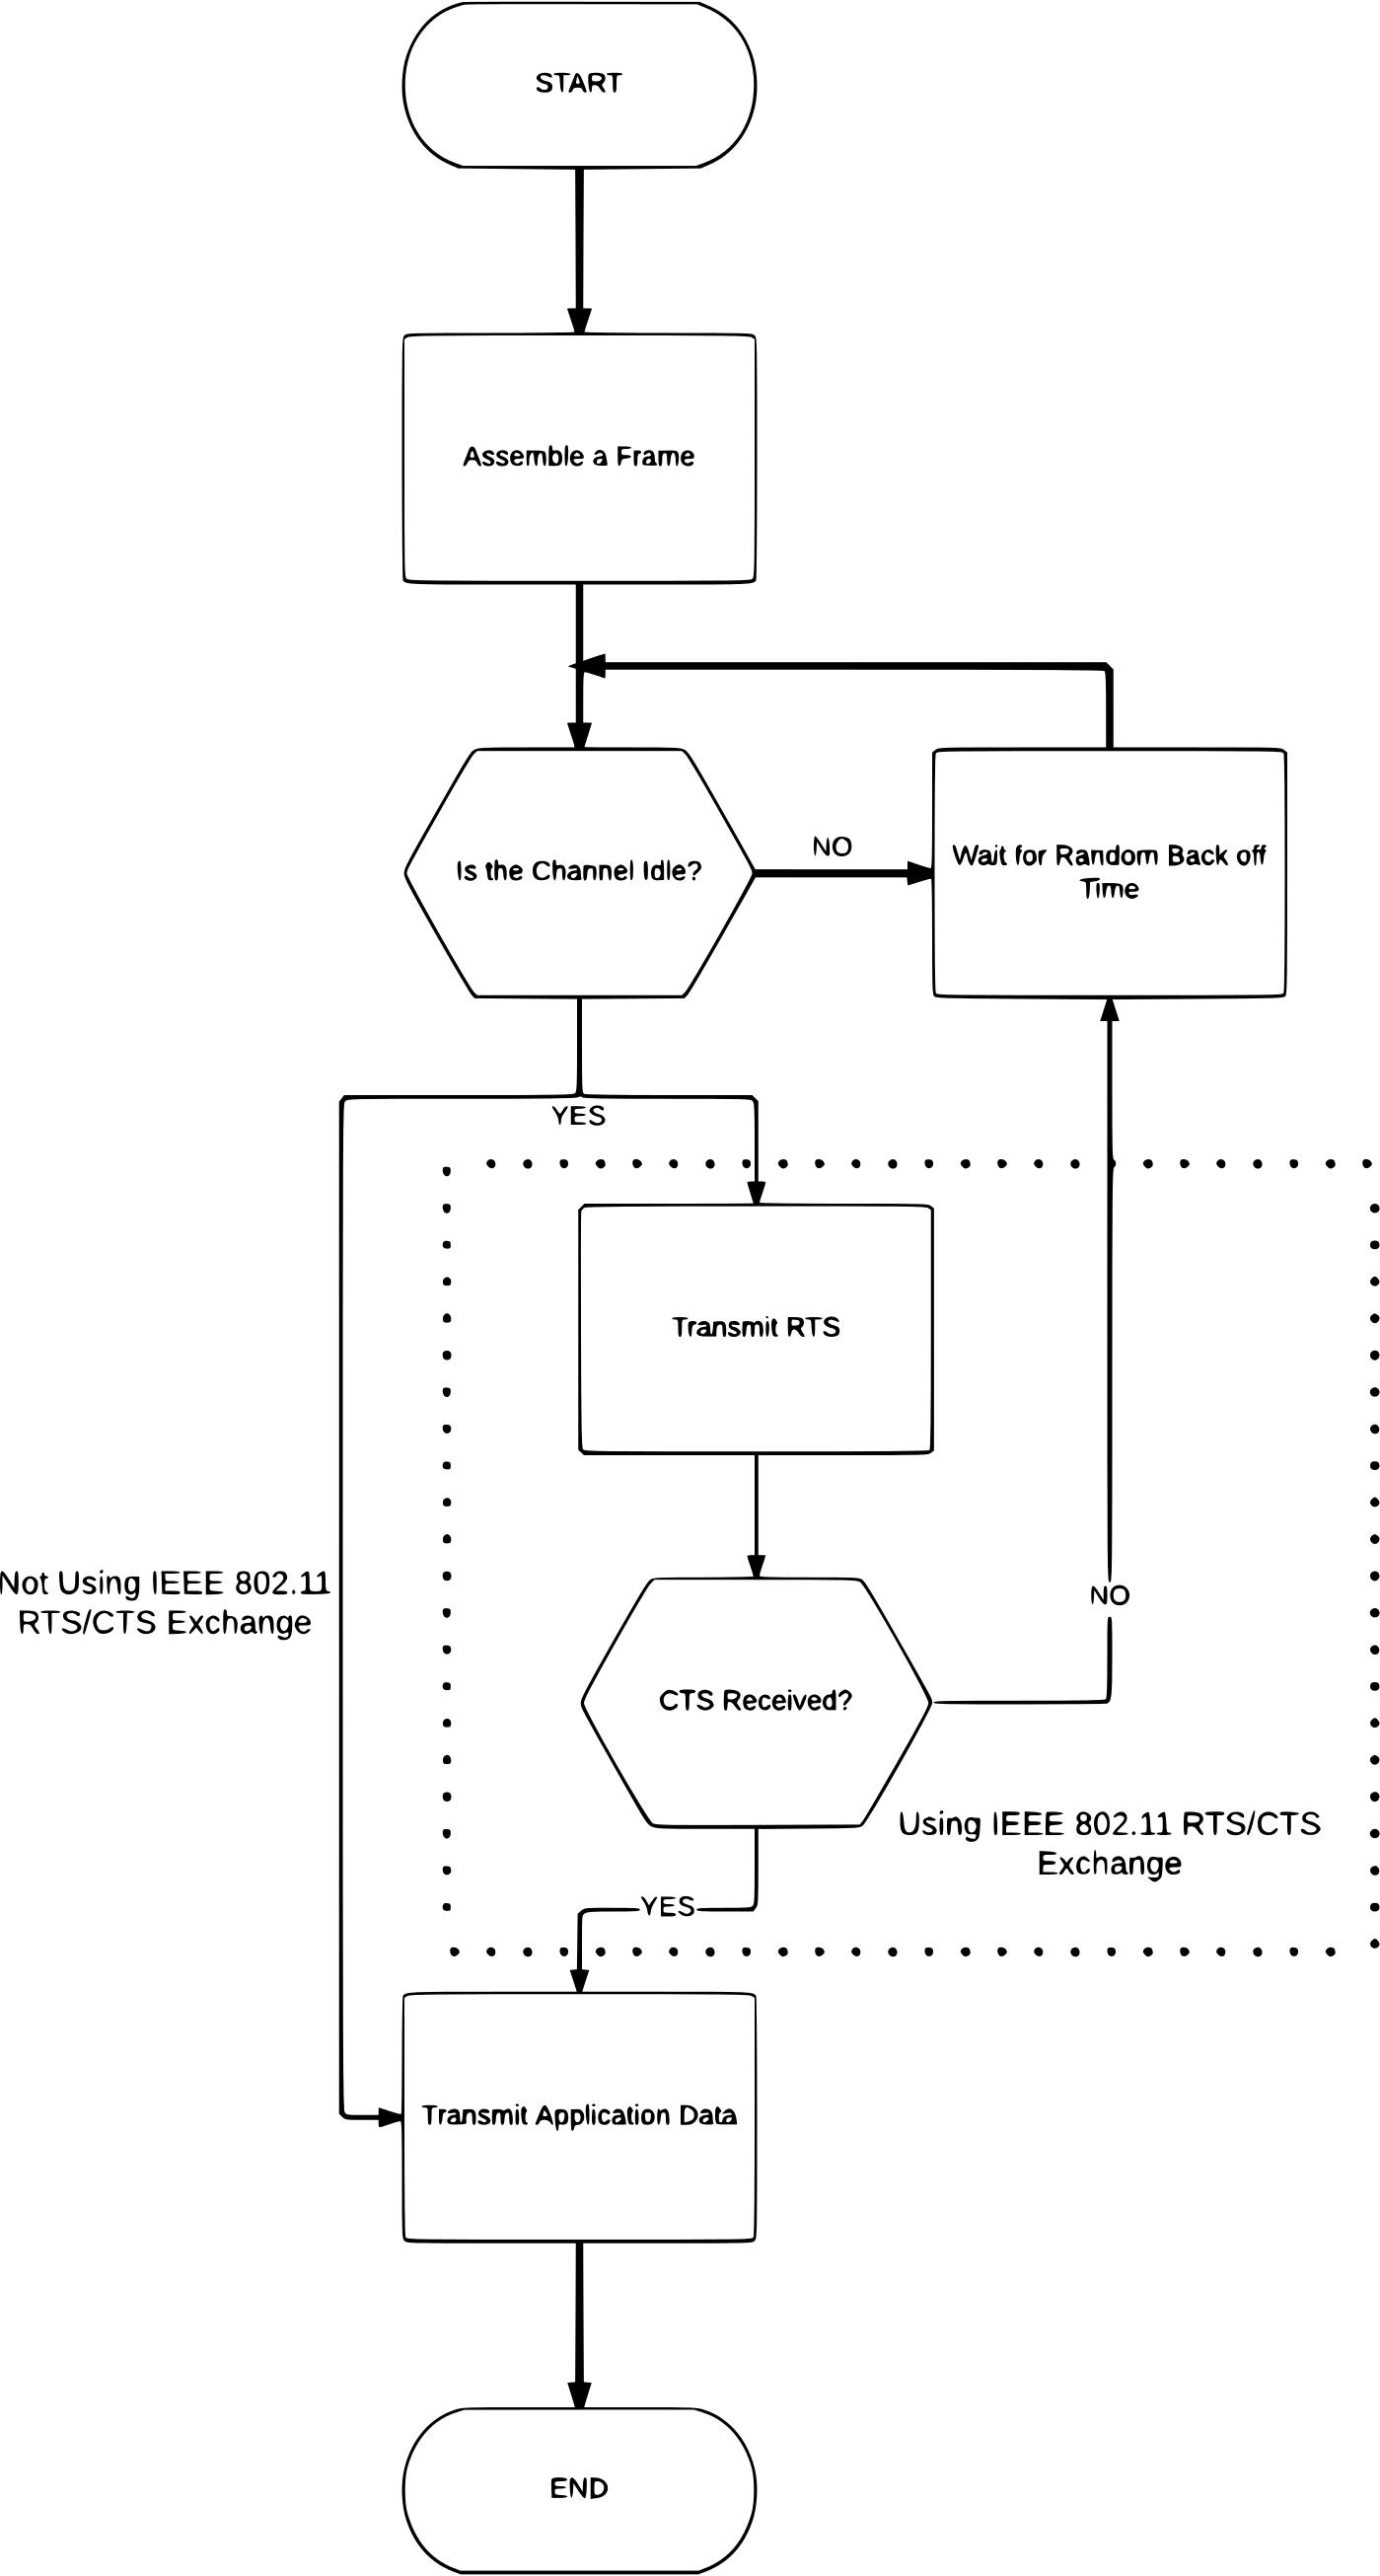
\includegraphics[height=.95\textheight]{csma-ca}
    \caption{Flowchart showing the operation of CSMA/CA. The dotted square shows RTS/CTS protocol, implementation of which is voluntary. RTS/CTS is part of 802.11 standard, but is not a part of 802.11b amendment. Source: \url{https://commons.wikimedia.org/wiki/File:Csma_ca.svg}}
    \label{fig:csma-ca}
\end{figure}
% 
\par // More info will follow here about how 802.11b is used in vehicular environment. I will investigate \cite{Bilgin2013PerformanceAreas}.

\subsubsection{802.11p} \label{sec:802.11p}
% 
802.11p is amendment to standard 802.11 by IEEE. This amendment was developed between 2005 and 2009 and was approved and published in 2010 as \enquote{Amendment 6: Wireless Access in Vehicular Environments}. It was included in 2012 revision of 802.11 and onwards.
802.11p is designed for vehicle-to-vehicle (V2V) and vehicle-to-infrastructure (V2I) communication. This communication can often exist for short period of time only, therefore some of the properties (such as authentication) defined by original 802.11 standards are omitted. The 802.11p has served as base for the ITS-G5 standard (described in next section).\par
% 
% 

\subsubsection{ETSI ITS-G5}
% http://www.etsi.org/deliver/etsi_en/302600_302699/302663/01.02.00_20/en_302663v010200a.pdf
ITS-G5 is a Dedicated Short Range Communication (DSRC) standard, running on the 5GHz frequency band based on \hyperref[sec:802.11p]{802.11p} in Europe.
The spectrum allocated for DSRC is 5.875-5.905 GHz also called ITS-G5A. This allocated spectrum of 30 MHz is only for ITS. Of the 30 MHz only a third of that is saved for the Road safety as seen on the picture below.\par
% 
The protocol stack for ETSI ITS G5 uses IEEE 802.11p as the physical layer. By dividing channels into Control Channel (CCH) and Service Channel (SCH), packets transmit through the control channel do not have to compete with service channel. For Medium access layer, channel access and priority is done by Enhanced Distributed Channel Access (EDCA) by using a variation of CSMA/CA. The packets not only compete for channel access with other vehicles but also with packets internally in the same node. Packets are divided by 4 access categories, VO, VI, BE and BK. Each access categories can be given one of the two channel types, resulting in 8 different combinations. Internal congestion control is being done (one for CCH and one for SCH) before the packet is sent to their respective queue. ETSI ITS G5 also performs a Decentralised Congestion Control (DCC), which changes transmit power, the minimum packet interval, the data rate, and the sensitivity of the radio accordingly. It does this by acting like a state machine going from a “active”, “relaxed” and “restrictive” state depending on the situation.
ETSI ITS G5 periodically transmit broadcast message called CAMs with information about their current state, location, speed, and direction with a frequency of 10 Hz.\par
% 
As described in conference proceedings for IEEE 79th Vehicular Technology Conference: \textquote[\cite{Shi2014SpectrumSafety}]{\textit{We performed extensive simulation for CSMA/CA and STDMA MAC (Simulation parameters) schemes in an urban highway scenario with realistic traffic density. Results show that more than 80 MHz is required to achieve 1\% packet loss with 500 m communication range. It is significantly larger than the current spectrum allocated of 10 MHz in the US and Europe.}}\par 
% 
It is also mentioned that by decreasing the communication range to 100 m, the spectrum requirement is reduced to 20 MHz, still being twice the amount available today. 

\subsubsection{ARIB STD-T109}
% 
% Section about Japanese technology ARIB.
% 
% Some info: \url{http://www.arib.or.jp/english/html/overview/doc/5-STD-T109v1_0-E1.pdf} and \url{http://www.ccs-labs.org/bib/heinovski2016performance/heinovski2016performance.pdf}
% 
The radio communication requirements for ARIB consist of single channel radio communication in the 700 MHz band with both V2I and V2V communication. The communication have to support V2V communication up to 140 km/h and V2I up to 70 km/h.\par
% 
The protocol stack of ARIB STD-t109 is from the bottom, the physical layer based on IEEE 802.11p. Above the physical layer is the MAC (Medium access layer) with a combination of TDMA and CSMA/CA channel access. The next layer is the IVC-RVC layer, which controls the channel access parameters, synchronises clocks, and handles communication control. Lastly is the layer 7 and application layer which is for the communication with users and for security.\par
% 
Though ARIB is using a physical layer like IEEE 802.11p, one of the key differences is that the MAC distinguishes between communication traffic between IVC (Vehicle to vehicle) and RVC (Vehicle to infrastructure). The TDMA scheme is used by having control cycles of 100.000$\upmu$s which is then divided into 16 smaller cycles of  6240$\upmu$s. Each of the small cycles have 2 periods, the first period, 0 to 3024$\upmu$s is called RVC period which is the period where only V2I is allowed to access the channel. The reason is that the infrastructures is connected to multiple sensors scattered around the road, giving it more knowledge about the current situation than a vehicle for distributing safety information. Since each infrastructure can be allocated a specific time-slot in the RVC period, it is not necessary to use CSMA/CA. After the RVC period ends (after 3024$\upmu$s), vehicles can compete for channel access, but to avoid concurrent channel access with other vehicles, CSMA/CA is used \cite{Heinovski2016PerformanceSTD-T109}.\par
% 
Like the 802.11p and ETSI, ARIB also uses OFDM (Orthogonal Frequency Division 
Multiplexing) as modulation scheme. OFDM uses BPSK, QPSK, 16-QAM and 64-QAM \footnotemark.\par
% 
\footnotetext{\url{http://rfmw.em.keysight.com/wireless/helpfiles/n7617a/coding_and_modulation.htm}, accessed on 17/04/2017}
% 
% 
ARIB using both TDMA and CSMA/CA (compare to 802.11p only using CSMA/CA) gives it a better communication distance in urban environment almost up to 3 times the distance \cite{Heinovski2016PerformanceSTD-T109}, because it suffers less from obstacles such as buildings etc. On the other hand, because of the priority of the RVC period, it causes packet losses for the traffic between vehicles. For same reason, message delays also happens, since they need to wait for the next time slot, which is not reserved, this causes delay in ms. 